\section{Experiments}
\label{sec:exp}

\paragraph{Setup and pre-registration.} Testbed-A is 2D: \texttt{two\_moons}
(the connected-manifold task where a censored tail is reachable by short
extrapolation \emph{along} the manifold) plus \texttt{eight\_gaussians} and
\texttt{pinwheel} for the estimation checks. The selector $s_\beta(x)=\sigma(-\beta
x_1^{\mathrm{std}})$ is swept over the pre-registered grid $\beta\in\{0,0.5,1,2,
4,8\}$ at $5$ seeds; the censored slice is the fixed region $x_1^{\mathrm{std}}>
0.5$. The downstream model is an MLP; the augmentation budget ($2000$ synthetic
units) is matched across every generative method. The beta grid, seeds, the one
operating point ($\gamma{=}6$ plus quantile gate rules), and every
kill-condition threshold were committed in \texttt{PLAN.md} \emph{before} the
results commit. Baselines span B0 (obs-only floor), B1 (SMOTE), B2 and a
diversity-matched B2, B3 ($1/\shat$ reweighting --- the central squeeze), and B4
(oracle on the full population); the sharp control is the misdirected selector
at matched guidance strength.

\begin{figure}[t]
\centering
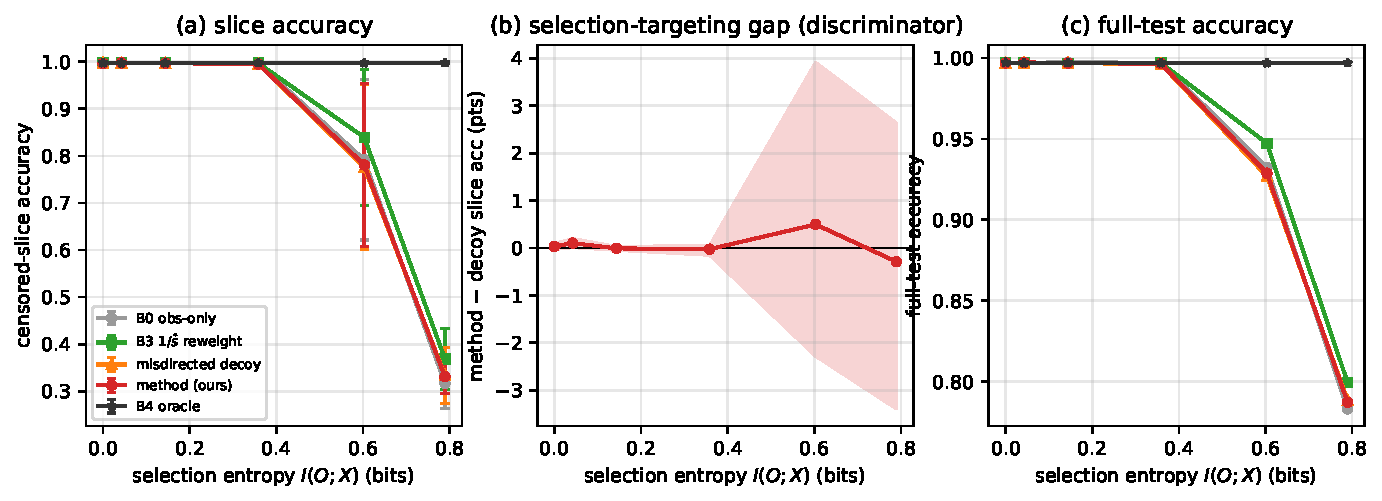
\includegraphics[width=\textwidth]{figs/fig1_curve.pdf}
\caption{The go/no-go curve. (a) Censored-slice accuracy vs selection entropy:
once censoring bites, no on-support method (method, decoy, B3) closes the gap to
the oracle B4. (b) The pre-registered discriminator --- method$-$decoy slice gap
--- stays at zero within its bootstrap band across the whole entropy range (K1
negative). (c) Full-test accuracy. Selection targeting does not become a
downstream advantage over the matched decoy.}
\label{fig:curve}
\end{figure}

\subsection{E0: the selector is recovered, on the complement too}
\label{sec:e0}
Across all three testbeds and every $\beta>0$, the calibrated ensemble recovers
$s_\beta$ with global Spearman $\ge\EZeroRhoGlobalMin$ and --- the region-split
check that guards against the silent false-GO --- \emph{complement} Spearman
$\ge\EZeroRhoCompMin$, at ECE $\le\EZeroEceMax$ (Fig.~\ref{fig:e0}). The plug-in
selection entropy from $\shat$ tracks the analytic value across $\beta$ at
correlation $\EZeroIOXCorr$, and is $\IOXZero$ at $\beta{=}0$ (MCAR) rising to
$\IOXEight$ at $\beta{=}8$. Estimation is not the bottleneck.

\begin{figure}[t]
\centering
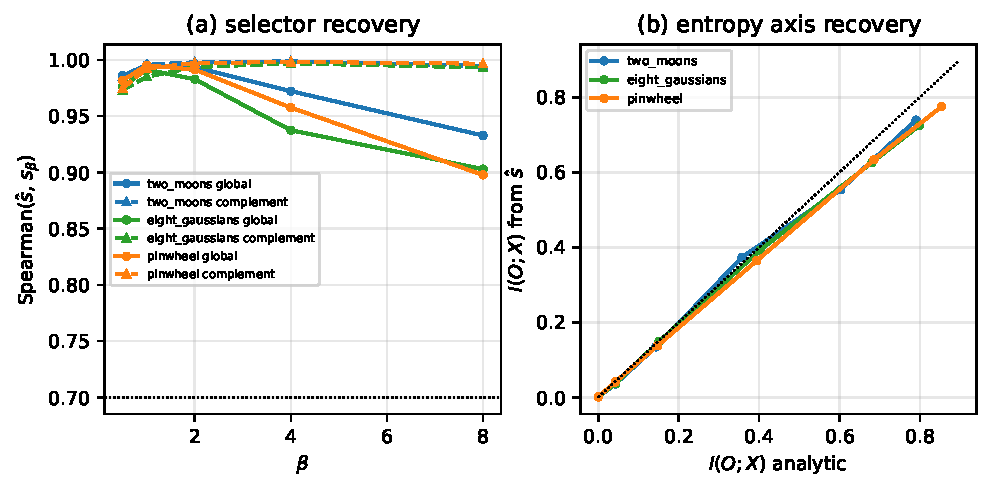
\includegraphics[width=\textwidth]{figs/fig2_e0.pdf}
\caption{E0. (a) The calibrated ensemble recovers $s_\beta$ globally
\emph{and} on the complement across all three testbeds (dashed line at the
$0.7$ gate). (b) Plug-in $\IOX$ from $\shat$ tracks the analytic value.}
\label{fig:e0}
\end{figure}

\subsection{E1: the bridge targets the censored complement}
\label{sec:e1}
The bridge does its job as a generator. At $\beta{=}4$ the synthesized units land
in the on-manifold censored complement at rate $\EOneCompHitMethod$, versus
$\EOneCompHitDecoy$ for the misdirected decoy and $\EOneCompHitBTwo$ for
selection-agnostic sampling --- selection targeting roughly doubles the
complement-hit rate --- while the independent density/NN validator rejects only
$\EOneRejectMethod$ of synthesized units as off-manifold (Fig.~\ref{fig:collar}).
The mechanism locates and fills the right region.

\begin{figure}[t]
\centering
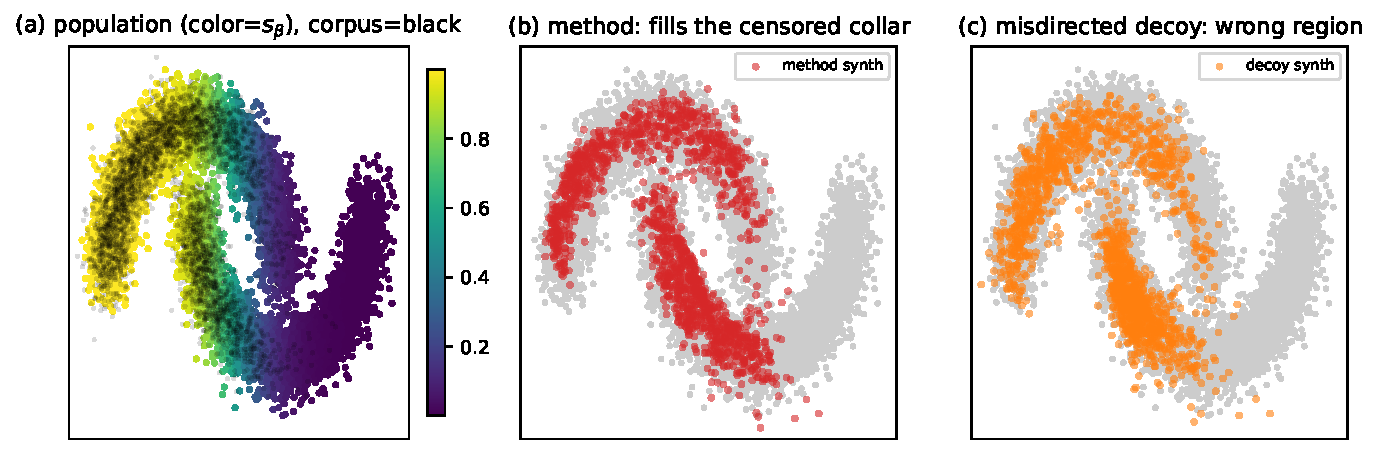
\includegraphics[width=\textwidth]{figs/fig3_collar.pdf}
\caption{The bridge targets the censored complement ($\beta{=}4$). (a) Population
colored by the true selection $s_\beta$; the curated corpus (black) is thinned in
the high-$x_1$ tail. (b) The method's synthesized units concentrate in the
low-$s$ collar. (c) The matched misdirected decoy places identically-strong
guidance in the wrong region.}
\label{fig:collar}
\end{figure}

\subsection{E2: targeting does not become a downstream advantage (the negative)}
\label{sec:e2}
Here the pre-registered go/no-go fails (Fig.~\ref{fig:curve};
Table~\ref{tab:e2}). The left end is clean: at $\beta{=}0$ the method's
slice gain over B0 is $\LeftEndGain$ points (CI $\LeftEndGainCI$) and the
method$-$decoy gap is $\LeftEndGap$ --- nothing to recover under MCAR, as the
theorem requires. But the discriminating quantity never lifts off:
\begin{itemize}
\item \textbf{K1 (trend).} The method$-$decoy slice gap does not rise with
selection entropy: Spearman$(\text{gap},\IOX)=\KOneSpearman$
($p{=}\KOneSpearmanP$, one-sided), and the $\beta{=}8$-vs-$\beta{=}0$ gap fails
the paired Wilcoxon ($p{=}\KOneWilcoxonP$).
\item \textbf{K2 (matched decoy).} At $\beta{=}8$ the method does not exceed the
misdirected decoy on the slice ($p{=}\KTwoMethodVsDecoyP$, effect
$\KTwoMethodVsDecoyEff$), nor clear the diversity-matched B2
($p{=}\KTwoMethodVsBTwoDivP$).
\item \textbf{Versus reweighting.} The method \emph{trails} $1/\shat$
reweighting by $\MethodVsBThreeGap$ points at $\beta{=}8$
($p{=}\MethodVsBThreeP$).
\end{itemize}
The synthesized units are correctly labeled (label purity $>0.99$; the negative
is not a mislabeling artifact) and pass the off-manifold validator (reject
$\MethodRejectHi$ at $\beta{=}8$). Selection targeting is real; its downstream
payoff, measured against the matched decoy, is not.

\begin{table}[t]
\centering\small
\caption{Censored-slice accuracy (\%, mean over 5 seeds). Generation (method,
decoy) neither beats the obs-only floor B0 nor $1/\shat$ reweighting (B3) once
censoring bites ($\beta\ge4$); the huge B4 gap is headroom nobody on-support can
reach. The method$-$decoy gap (last column) never separates from zero relative
to its seed spread.}
\label{tab:e2}
\begin{tabular}{lrrrrrrr}
\toprule
$\beta$ & $\IOX$ & B0 & B3 rew. & decoy & method & B4 oracle & method$-$decoy \\
\midrule
0 & \IOXZero & \SliceBzeroZero & \SliceBrewZero & \SliceDecoyZero & \SliceMethodZero & \SliceBoracleZero & $\GapZero$ \\
2 & \IOXTwo & \SliceBzeroTwo & \SliceBrewTwo & \SliceDecoyTwo & \SliceMethodTwo & \SliceBoracleTwo & $\GapTwo$ \\
4 & \IOXFour & \SliceBzeroFour & \SliceBrewFour & \SliceDecoyFour & \SliceMethodFour & \SliceBoracleFour & $\GapFour$ \\
8 & \IOXEight & \SliceBzeroEight & \SliceBrewEight & \SliceDecoyEight & \SliceMethodEight & \SliceBoracleEight & $\GapEight$ \\
\bottomrule
\end{tabular}
\end{table}

\subsection{The central squeeze: why targeting does not pay}
\label{sec:squeeze}
Fig.~\ref{fig:squeeze} is the paper's finding. Binning test points by
distance-from-observed-support and by $\shat$ epistemic uncertainty, the
(method $-$ B3) accuracy advantage is a bounded ridge: near the observed support
$\shat$ is reliable and reweighting already captures the signal, so generation
adds nothing; far into the complement $\shat$ is off-support extrapolation and
the identifiability gates forbid steering, so generation is absent. Between them
is a thin collar where generation could in principle help --- but on this task
that collar carries little residual headroom over B3, and its width is set by
$\shat$ reliability, not by how much censored mass exists. This is the squeeze
the design anticipated, now measured: \emph{generation buys at most a bounded
collar beyond reweighting, and here the collar is too narrow to win}.

\begin{figure}[t]
\centering
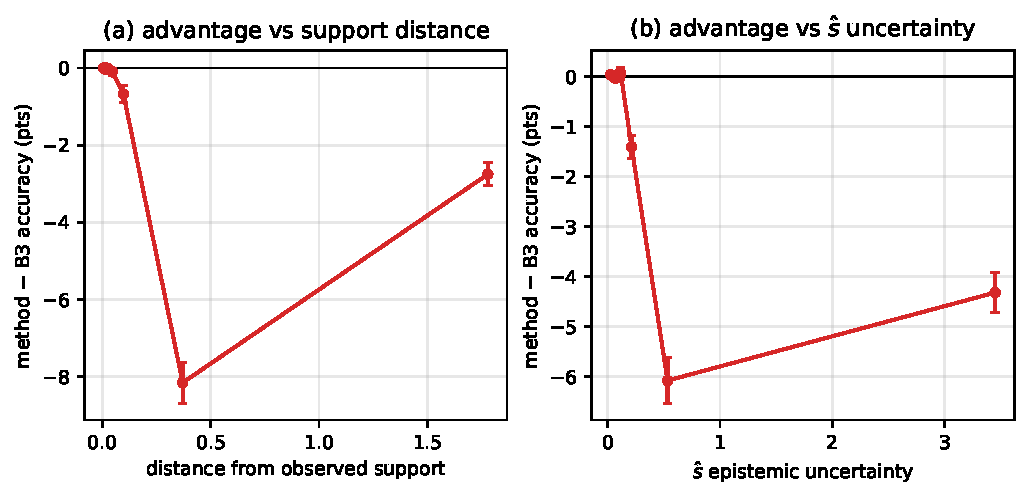
\includegraphics[width=0.86\textwidth]{figs/fig4_squeeze.pdf}
\caption{The central squeeze. The (method $-$ B3 reweighting) accuracy advantage
against (a) distance from observed support and (b) $\shat$ epistemic
uncertainty. Near the support reweighting already wins; far into the complement
$\shat$ is untrustworthy and the gates forbid steering. The advantage lives, if
anywhere, in a thin collar between --- here too narrow to matter.}
\label{fig:squeeze}
\end{figure}

\subsection{Scope: the method fails on foreign structure, as it must (K4)}
\label{sec:scope}
A disconnected, non-recombinable satellite planted in the censored region is a
positive control: a method that recovered it would be leaking, not
generalizing. It does not. The method's gain on the foreign region is
$\KFourForeignGain$ points --- versus $\KFourCollarGain$ on the recombinable
collar --- and only $\KFourSynthInForeign$ of synthesis lands in the foreign
region (Fig.~\ref{fig:robust}a). The scope fence holds: the method recovers
censored \emph{combinations} of observed structure, not new structure.

\begin{figure}[t]
\centering
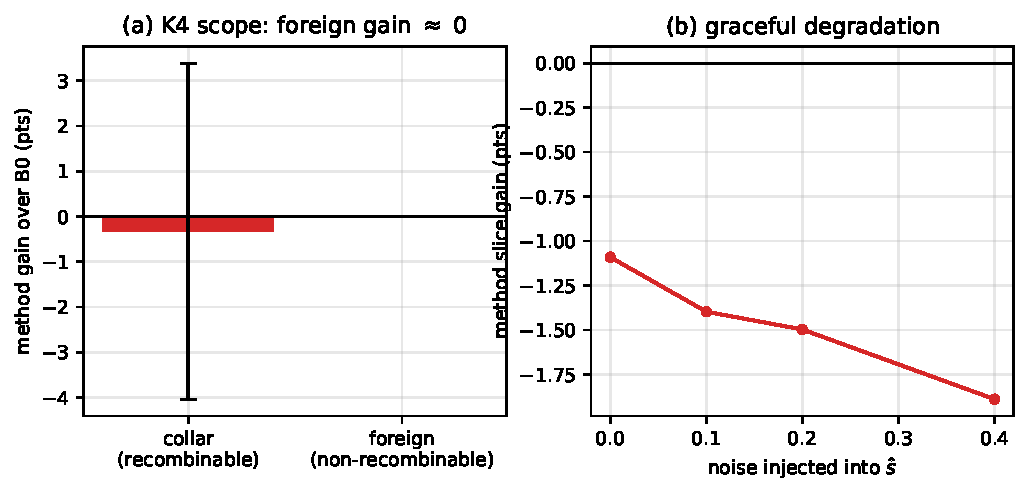
\includegraphics[width=0.86\textwidth]{figs/fig5_robust.pdf}
\caption{(a) K4 scope control: the method's gain over B0 on the recombinable
collar versus the planted non-recombinable foreign satellite, which it (correctly)
does not recover. (b) Injecting noise into $\shat$ monotonically worsens the
method's (already non-positive) slice effect.}
\label{fig:robust}
\end{figure}

\subsection{Robustness}
\label{sec:robust}
Consistent with the negative headline, the method's net effect on the slice at
$\beta{=}4$ is a slight loss even with clean $\shat$ ($\NoiseGainClean$ points),
and corrupting $\shat$ with noise only deepens it (to $\NoiseGainHi$ at the
highest level; Fig.~\ref{fig:robust}b) --- there is no positive gain for $\shat$
reliability to protect. The guidance-norm cap nonetheless remains load-bearing
for the off-manifold guard: removing it more than doubles the independent reject
rate ($\CapOnReject\to\CapOffReject$), confirming the guards do their job even
though the payoff does not materialize.

\subsection{The real-corpus limit and the perceptual rung}
\label{sec:real}
\paragraph{Real-corpus pilot (limits only).} As a limits check we curate a real
tabular corpus --- California housing, two standardized features, target
above-median value --- with a \emph{real} covariate driving the MNAR selection
($s_\beta$ on standardized median income, censoring high-income tracts), taking
the raw unfiltered pool as the reference cover. A cover-blind check confirms the
reference is not co-censored on the target region (the selector retains signal
there, slice $\shat$ spread $\EFiveCoverStd$; K5 not triggered). At strong
censoring the method attains $\EFiveSliceMethod$ slice accuracy versus
$\EFiveSliceBZero$ for the obs-only floor and $\EFiveSliceDecoy$ for the
misdirected decoy --- and here it \emph{does} beat $1/\shat$ reweighting
($\EFiveSliceBThree$), which becomes high-variance when a few heavily-censored
tail points carry enormous weights. The lesson is not that generation wins: the
method-minus-\emph{decoy} margin --- the selection-targeting signal --- remains
within noise, exactly as in 2D. It is that generation's advantage over
\emph{reweighting} is dataset-dependent (it appears precisely where reweighting
is ill-behaved), whereas its advantage over matched misdirected guidance is the
invariant, and invariantly small. We report this as characterization, not a
real-corpus go: three seeds, a synthetic-style selector on real features, and a
full-support reference cover a genuine corpus would not hand us.

\paragraph{The perceptual rung.} A faithful perceptual testbed (pixel-space
subpopulation censoring with an EDM/twisted-SMC bridge) is the natural next rung.
A cheap latent-space proxy we ran (PCA of MNIST with the same pipeline) was
uninformative on both ends --- the digit subpopulation the thickness selector
censors remains easily classifiable, so no downstream headroom exists to
contest, and a small latent diffusion is flagged off-manifold by the independent
validator --- so we do not report it as evidence and leave the faithful
pixel-space version, which the 2D and real-tabular findings already frame, to
future work.

